\documentclass[11pt,a4paper]{article}

% --- Typography & Fonts ---
\usepackage[utf8]{inputenc}
\usepackage[T1]{fontenc}
\usepackage[french]{babel}
\usepackage{charter} % Elegant and modern font
\usepackage[scaled=0.92]{helvet}
\usepackage{courier}
\usepackage{setspace}
\setstretch{1.15} % Better line spacing

% --- Math and Symbols ---
\usepackage{amsmath, amsfonts, amssymb}

% --- Graphics and Layout ---
\usepackage{graphicx}
\usepackage{geometry}
\usepackage{float}
\usepackage{titlesec}
\usepackage{fancyhdr}
\usepackage{geometry}
\geometry{
    a4paper,
    top=2.5cm,
    bottom=2.5cm,
    left=2.5cm,
    right=2.5cm,
    headheight=15pt
}

% --- Colors and Styling ---
\usepackage{xcolor}
\definecolor{MainBlue}{HTML}{003366}
\definecolor{AccentBlue}{HTML}{0055AA}
\definecolor{SlateGray}{HTML}{2D3E50}
\definecolor{LightGray}{HTML}{F8F9FA}
\definecolor{MintGreen}{HTML}{E8F5E9}
\definecolor{BorderGray}{HTML}{E0E0E0}

% --- Tables and Boxes ---
\usepackage{booktabs}
\usepackage{tabularx}
\usepackage{colortbl}
\usepackage{tcolorbox}
\tcbuselibrary{skins, breakable}

% --- Hyperlinks ---
\usepackage{hyperref}
\hypersetup{
    colorlinks=true,
    linkcolor=MainBlue,
    citecolor=AccentBlue,
    urlcolor=AccentBlue,
    pdftitle={Rapport d'Architecture Technique - Webmapping},
    pdfauthor={FOX Mapping Team}
}

% --- Section Styles ---
\titleformat{\section}
  {\color{MainBlue}\normalfont\Large\bfseries}
  {\thesection}{1em}{}[{\titlerule[1pt]}]

\titleformat{\subsection}
  {\color{SlateGray}\normalfont\large\bfseries}
  {\thesubsection}{1em}{}

% --- Header/Footer ---
\pagestyle{fancy}
\fancyhf{}
\fancyhead[L]{\small \textcolor{SlateGray}{Architecture Technique : Système de Webmapping}}
\fancyhead[R]{\small \textcolor{SlateGray}{\thepage}}
\fancyfoot[C]{\footnotesize \textcolor{gray}{Projet Webmapping SIG - Rapport Technique}}
\renewcommand{\headrulewidth}{0.5pt}
\renewcommand{\headrule}{\hbox to\headwidth{\color{MainBlue}\leaders\hrule height \headrulewidth\hfill}}

% --- Page de Garde ---
\begin{document}

\begin{titlepage}
    \centering
    \vspace*{1.5cm}
    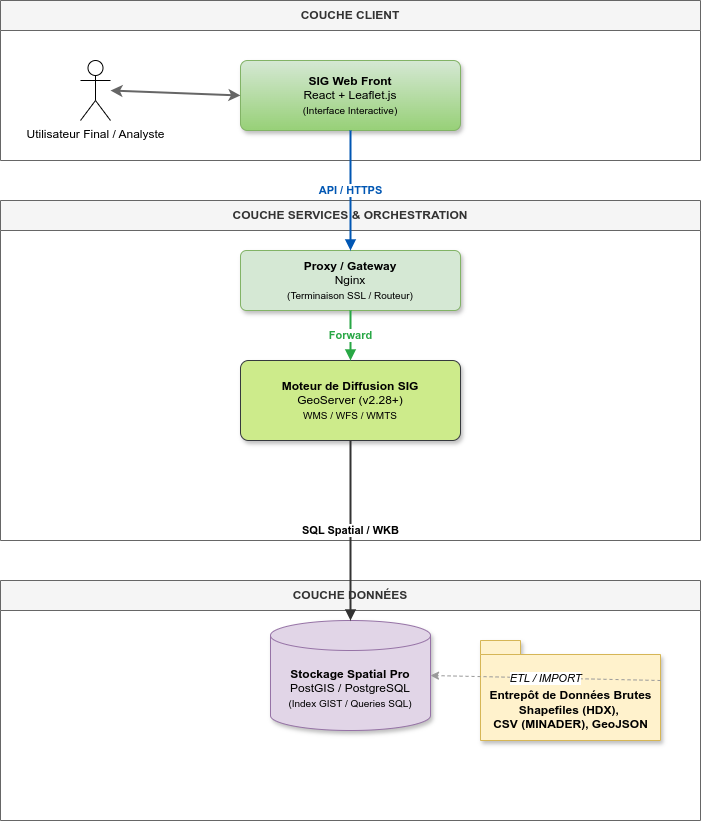
\includegraphics[width=0.25\textwidth]{architecture_diagram.png}\\[1cm]
    
    {\Huge \bfseries \textcolor{MainBlue}{Rapport d'Architecture Technique}}\\[0.8cm]
    {\Large \textcolor{SlateGray}{Système de Webmapping SIG pour le Suivi Agricole}}\\[1.5cm]
    
    \begin{tcolorbox}[colback=LightGray, colframe=MainBlue, width=0.8\textwidth, arc=2mm, boxrule=1pt]
        \centering
        \large \bfseries \textcolor{MainBlue}{Étude des Bassins de Production du Cameroun}
    \end{tcolorbox}
    
    \vfill
    
    \begin{minipage}{0.45\textwidth}
        \begin{flushleft} \large
            \textcolor{SlateGray}{\textbf{Équipe de Projet :}}\\
            FOX Mapping Team\\
            \small \textit{Janvier - Février 2026}
        \end{flushleft}
    \end{minipage}
    \begin{minipage}{0.45\textwidth}
        \begin{flushright} \large
            \textcolor{SlateGray}{\textbf{Statut :}}\\
            Document de Référence\\
            \small \textit{Version 1.2}
        \end{flushright}
    \end{minipage}

    \vspace{2cm}
\end{titlepage}

\newpage

% --- Résumé ---
\begin{tcolorbox}[colback=LightGray, colframe=MainBlue, title=Résumé, arc=0mm, fonttitle=\bfseries]
Ce document présente l'architecture technique détaillée du projet de Webmapping. Il décrit l'intégration des différents serveurs (PostGIS, GeoServer), le rôle du frontend React/Leaflet, ainsi que la stratégie de conteneurisation via Docker. Une attention particulière est portée sur la justification des choix technologiques pour assurer la performance, la scalabilité et la sécurité du système.
\end{tcolorbox}

\tableofcontents
\newpage
% --- Introduction ---
\section{Introduction}

\noindent \textbf{Contexte} \\
\indent Le Cameroun, souvent qualifié d'« Afrique en miniature » en raison de sa diversité agro-écologique, possède des bassins de production économique extrêmement variés. Des cultures de rente comme le cacao dans le Grand Sud aux vastes zones d’élevage bovin dans l'Adamaoua, chaque division administrative (10 régions, 58 départements) joue un rôle spécifique dans la sécurité alimentaire et l'économie nationale. La gestion efficace de ces ressources et la planification stratégique nécessitent une vision spatiale claire pour orienter les politiques de développement et optimiser l'exploitation des bassins de production.

\vspace{1.5em}
\noindent \textbf{Problématique} \\
\indent Malgré la richesse des données statistiques collectées par les organismes publics tels que le MINADER, le MINEPIA ou l'INS, leur exploitation reste souvent limitée par l'absence d'outils de visualisation interactive. Il est complexe pour les décideurs, les étudiants et les acteurs économiques de localiser précisément les principaux pôles de production, d'analyser les dominances par filière ou de comparer les performances inter-départementales uniquement via des tableaux statiques. Le manque de corrélation dynamique entre les données socio-économiques et les référentiels géographiques freine la compréhension fine des dynamiques territoriales.

\vspace{1.5em}
\noindent \textbf{Objectifs} \\
\indent L'objectif principal de ce projet est de concevoir et déployer une plateforme de Webmapping performante dédiée à la cartographie des bassins de production agricole, d'élevage et de pêche au Cameroun. Ce système vise à intégrer des données multi-thématiques dans une base de données spatiale PostGIS, de les diffuser via GeoServer selon les standards OGC (WMS/WFS), et de proposer une interface cartographique interactive intuitive basée sur React et Leaflet. La plateforme permettra de visualiser la production à différents niveaux administratifs, offrant ainsi un outil d'aide à la décision visuel et pédagogique.

% --- Phases du Projet ---
\section{Phases de Réalisation du Projet}
La mise en œuvre de ce système de Webmapping s'est articulée autour de quatre phases critiques, garantissant la cohérence entre les données métier et leur représentation spatiale.

\begin{enumerate}
    \item \textbf{Définition des Bassins :} Identification des filières dominantes par secteur (Agriculture : cacao, maïs ; Élevage : bovins, volailles ; Pêche : zones littorales et continentales) et association aux divisions administratives correspondantes.
    \item \textbf{Collecte et Structuration :} Acquisition des fonds de carte (Shapefiles des régions et départements) et des données de production, suivie de leur nettoyage pour assurer l'intégrité du système.
    \item \textbf{Ingénierie des Données :} Mise en place de la base de données PostGIS, création des entités spatiales (polygones) et jointures avec les attributs de production.
    \item \textbf{Développement Web-Mapping :} Configuration du serveur SIG (GeoServer) pour la publication des services et création de l'interface utilisateur interactive avec filtres dynamiques et légendes adaptatives.
\end{enumerate}
% --- Schéma Directeur ---
\section{Schéma Directeur de l'Architecture}
L'architecture suit un modèle client-serveur robuste. Elle est conçue pour être hautement scalable, sécurisée et pédagogique. Le fonctionnement global repose sur un flux de données descendant, partant de la base de données centrale vers l'interface de visualisation finale.

\begin{figure}[H]
    \centering
    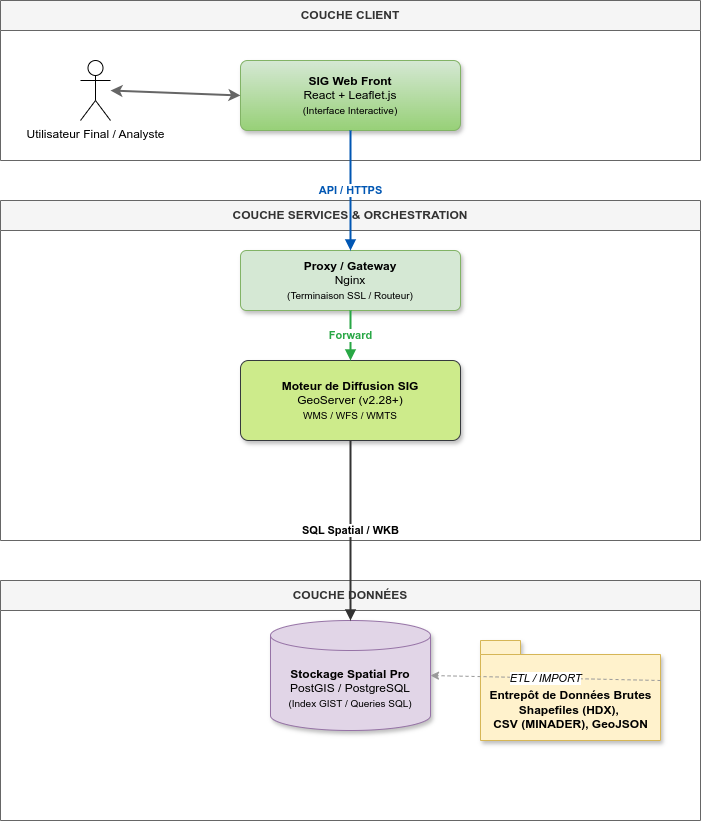
\includegraphics[width=0.85\textwidth]{architecture_diagram.png}
    \caption{Schéma Directeur : Flux de données entre les couches Client, Service et Données}
    \label{fig:schema_directeur}
\end{figure}

% --- Backend ---
\section{Composantes du Backend}

\subsection{Base de Données Spatiale : PostGIS}
La couche de persistance des données spatiales est assurée par \textbf{PostGIS}, une extension avancée du système de gestion de base de données relationnelle PostgreSQL.

PostGIS constitue le \textbf{standard de facto de l’écosystème open-source SIG}. Il offre des performances exceptionnelles grâce à l’utilisation \textbf{d’index spatiaux de type GiST} (Generalized Search Tree), permettant de manipuler efficacement des jeux de données contenant des millions de géométries complexes.

\textbf{Fonctionnalités principales :}
\begin{itemize}
    \item Stockage et gestion optimisée des données vectorielles (points, lignes, polygones).
    \item Exécution de requêtes spatiales complexes (intersection \texttt{ST\_Intersects}, buffers, jointures spatiales).
    \item Compatibilité native avec les référentiels de coordonnées standards (EPSG).
    \item Communication bidirectionnelle avec le serveur SIG pour la publication des couches.
\end{itemize}

\subsection{Serveur de Cartographie : GeoServer}
\textbf{GeoServer} joue le rôle de pivot dans l’architecture backend. Il assure la transformation des données brutes en services web utilisables par les applications clientes.

Il agit comme une \textbf{couche intermédiaire intelligente} en exposant les données selon les standards internationaux de l’Open Geospatial Consortium (OGC).

\textbf{Fonctionnalités principales :}
\begin{itemize}
    \item \textbf{Web Map Service (WMS)} : Génération dynamique de tuiles cartographiques raster.
    \item \textbf{Web Feature Service (WFS)} : Exposition des données géographiques vectorielles (GeoJSON).
    \item \textbf{Moteur de Rendu} : Séparation du fond et de la forme via le langage \textbf{SLD} (Styled Layer Descriptor).
    \item \textbf{Sécurité Applicative} : Gestion fine des droits d'accès par couche et par service.
\end{itemize}

\subsection{Reverse Proxy : Nginx}
Un serveur \textbf{Nginx}, déployé dans un conteneur dédié, fait office de porte d'entrée unique (Reverse Proxy) devant GeoServer.

\textbf{Responsabilités principales :}
\begin{itemize}
    \item Sécurisation des flux via la terminaison SSL/TLS (HTTPS).
    \item Protection du moteur SIG en masquant l'architecture interne.
    \item Optimisation des performances par la mise en cache et l'équilibrage de charge.
\end{itemize}
\begin{figure}[H]
    \centering
    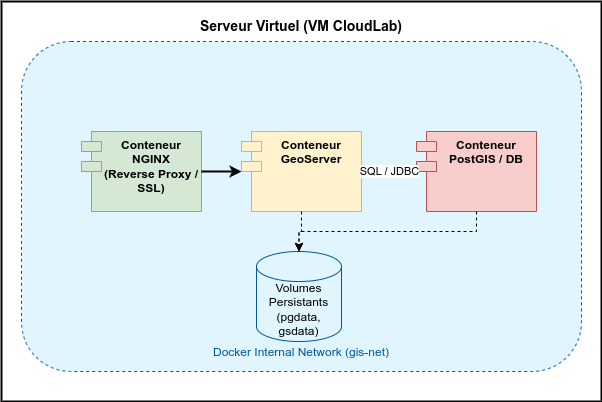
\includegraphics[width=0.85\textwidth]{network_architecture.png}
    \caption{Architecture Réseau : Segmentation des services par conteneurs Docker}
    \label{fig:architecture_reseau}
\end{figure}

% --- Conteneurisation ---
\section{Conteneurisation et Déploiement}
Pour garantir la portabilité et la reproductibilité totale du système, l’ensemble du backend est \textbf{conteneurisé à l’aide de Docker}. Cette approche permet d’assurer un comportement rigoureusement identique entre les environnements de développement et de production.

\subsection{Orchestration avec Docker Compose}
Un fichier \texttt{docker-compose.yml} orchestre les services PostGIS, GeoServer et Nginx sur un réseau virtuel privé.

\begin{itemize}
    \item \textbf{Isolation} : Chaque service opère dans son propre environnement sans conflit de dépendances.
    \item \textbf{Persistance} : Utilisation de volumes Docker externes pour garantir l'intégrité des bases de données lors des mises à jour.
    \item \textbf{Agilité} : Déploiement et arrêt de l'infrastructure complète via une commande unique, optimisant le temps de maintenance.
\end{itemize}

% --- Configuration Détaillée ---
\section{Configuration Détaillée de l'Infrastructure}

Cette section détaille les configurations spécifiques appliquées à chaque composant pour assurer leur interaction fluide au sein de l'environnement conteneurisé.

\subsection{Orchestration Globale (Docker Compose)}
Le fichier \texttt{docker-compose.yml} est le cœur de l'orchestration. Il définit trois services interconnectés sur un réseau bridge dédié \texttt{gis-net}.

\begin{tcolorbox}[colback=white, colframe=SlateGray, title=Extrait de la configuration Docker Compose]
\begin{verbatim}
services:
  postgis:
    image: postgis/postgis:16-3.4
    volumes:
      - pgdata:/var/lib/postgresql/data
      - ./postgis/init/:/docker-entrypoint-initdb.d # Scripts init
    networks:
      - gis-net

  geoserver:
    image: docker.osgeo.org/geoserver:2.28.0
    environment:
      - PROXY_BASE_URL=http://your_vm_ip/geoserver
    depends_on:
      - postgis
    networks:
      - gis-net

  nginx:
    image: nginx:alpine
    ports:
      - "80:80"
    depends_on:
      - geoserver
    networks:
      - gis-net
\end{verbatim}
\end{tcolorbox}

\subsection{Configuration de PostGIS}
L'initialisation de la base de données est automatisée. Au premier démarrage du conteneur, tous les scripts \texttt{.sql} et \texttt{.sh} présents dans le dossier \texttt{./postgis/init/} sont exécutés par ordre alphabétique.
\begin{itemize}
    \item \textbf{Schéma} : Les tables sont créées automatiquement avec les types spatiaux appropriés (\texttt{Geometry}, \texttt{SRID 4326}).
    \item \textbf{Données} : L'importation massive des données agricoles et géographiques est réalisée via des commandes \texttt{COPY} optimisées.
\end{itemize}

\subsection{Configuration de GeoServer}
GeoServer est configuré pour écouter derrière un proxy. La variable d'environnement \texttt{PROXY\_BASE\_URL} est critique : elle assure que les liens générés par GeoServer (notamment dans les documents \texttt{GetCapabilities}) pointent correctement vers l'adresse publique du serveur et non son adresse IP docker interne.

\subsection{Configuration Nginx (Reverse Proxy)}
Nginx agit comme une passerelle frontale. Sa configuration est minimale mais essentielle pour router le trafic vers GeoServer securiser.

\begin{tcolorbox}[colback=white, colframe=SlateGray, title=Configuration Nginx (nginx.conf)]
\begin{verbatim}
server {
    listen 443 ssl;
    server_name c220g2-011025.wisc.cloudlab.us;

    ssl_certificate /etc/letsencrypt/live/c220g2-011025.wisc.cloudlab.us/fullchain.pem;
    ssl_certificate_key /etc/letsencrypt/live/c220g2-011025.wisc.cloudlab.us/privkey.pem;

    root /usr/share/nginx/html;

    # Reverse proxy vers GeoServer
    location /geoserver/ {
        proxy_pass http://geoserver:8080/geoserver/;
        proxy_set_header Host $host;
        proxy_set_header X-Real-IP $remote_addr;
        proxy_set_header X-Forwarded-For $proxy_add_x_forwarded_for;
        proxy_set_header X-Forwarded-Proto $scheme;
        proxy_redirect off;

        # CSP permissif pour Wicket/PostGIS
        add_header Content-Security-Policy "default-src 'self'; script-src 'self' 'unsafe-inline' 'unsafe-eval'; style-src 'self' 'unsafe-inline'; img-src 'self' data:; form-action 'self' https://$host/geoserver;" always;
    }

    # Nginx static files (HTML pour test)
    location / {
        try_files $uri $uri/ =404;
    }
}
\end{verbatim}
\end{tcolorbox}

% --- Frontend ---
\section{GEO-Front — Géoportail Cameroun}

Interface cartographique de visualisation des données agricoles, d'élevage et de pêche au Cameroun.
\begin{figure}[H]
    \centering
    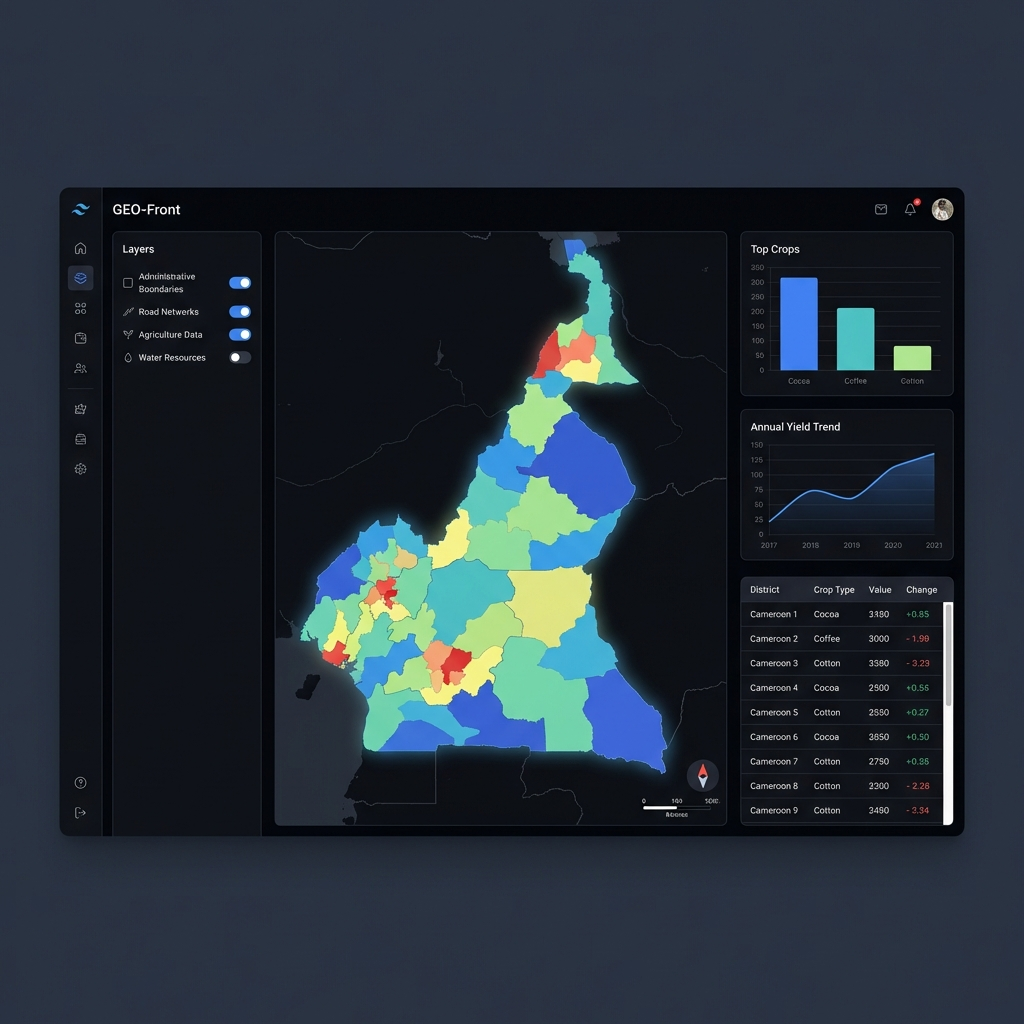
\includegraphics[width=0.95\textwidth]{geofont.png}
    \caption{Interface GEO-Front : Visualisation thématique et interactive (Mode Sombre)}
    \label{fig:apercu_frontend}
\end{figure}

\subsection{Vue d'ensemble}
\textbf{GEO-Front} est un géoportail web moderne permettant de visualiser et analyser les données de production agricole, d'élevage et de pêche du Cameroun. L'application offre deux modes de visualisation :

\begin{enumerate}
    \item \textbf{Vue Carte} : Analyse thématique choroplèthe sur fond de carte interactif.
    \item \textbf{Vue Tabulaire} : Matrice pivot avec données croisées années/zones.
\end{enumerate}

\subsubsection*{Stack Technique}
\begin{itemize}
    \item \textbf{Frontend} : React 18 + TypeScript + Vite
    \item \textbf{Cartographie} : React-Leaflet + Leaflet
    \item \textbf{Styles} : Tailwind CSS 4.x (dark mode natif)
    \item \textbf{Animations} : Framer Motion
\end{itemize}

\subsection{Données Disponibles}

\subsubsection*{Matrice de Disponibilité}
\begin{table}[H]
    \centering
    \small
    \renewcommand{\arraystretch}{1.2}
    \begin{tabularx}{\textwidth}{|l|l|l|l|X|}
    \hline
    \rowcolor{NavyBlue} \textcolor{white}{\textbf{Secteur}} & \textcolor{white}{\textbf{Granularité}} & \textcolor{white}{\textbf{Années}} & \textcolor{white}{\textbf{Source}} & \textcolor{white}{\textbf{État}} \\ \hline
    \textbf{Agriculture} & Département & 1998 - 2022 & MINADER/DESA & Complet \\ \hline
    \textbf{Élevage} & National & 2015 - 2021 & MINEPIA & Complet \\ \hline
    \textbf{Élevage} & Régional & 2020 - 2021 & MINEPIA & Partiel \\ \hline
    \textbf{Élevage} & Département & - & - & Indisponible \\ \hline
    \textbf{Pêche} & National & 2021 & MINEPIA & Complet \\ \hline
    \textbf{Pêche} & Régional (Infra.) & 2021 & MINEPIA & Complet \\ \hline
    \textbf{Pêche} & Département & 2021 & MINEPIA & Complet \\ \hline
    \end{tabularx}
    \caption{Disponibilité des données par secteur}
\end{table}

\subsubsection*{Filières Couvertes}
\noindent \textbf{Agriculture (23 cultures) :} Maïs, Manioc, Cacao, Café, Banane Plantain, Sorgho, Riz, Haricot, Arachide, Igname, Patate douce, Pomme de terre, Coton, Hévéa, Palmier à huile, Agrumes, Tomate, Oignon, Ail, Piment, Gombo, Ananas, Avocat.

\vspace{0.5em}
\noindent \textbf{Élevage (5 espèces) :} Bovins, Ovins, Caprins, Porcins, Volailles.

\vspace{0.5em}
\noindent \textbf{Pêche (4 types + 6 infrastructures) :}
\begin{itemize}
    \item Types : Pêche Artisanale Maritime, Pêche Continentale, Pêche Industrielle, Pisciculture.
    \item Infrastructures : Débarcadères, Halls de vente, Fumoirs, Étangs actifs, Cages, Bacs.
\end{itemize}

\subsection{Fonctionnalités Actuelles}
\begin{itemize}
    \item \textbf{Interface Générale} : Responsive mobile-first, Thème sombre "True Black", Animations fluides.
    \item \textbf{Sidebar / Panneau de Contrôle} : Sélection du secteur, niveau administratif, et liste filtrée des filières.
    \item \textbf{Vue Carte} : 5 fonds de carte, synchronisation thème, choroplèthe dynamique, panneau info au survol.
    \item \textbf{Vue Tabulaire} : Pivot table, sélecteur de région, tendances visuelles.
\end{itemize}

\subsection{Fonctionnalités Planifiées}
\begin{itemize}
    \item \textbf{Carte} : Propagation niveau admin, couche limites seule, outils Leaflet (mesure, plein écran).
    \item \textbf{Données} : Intégration GeoServer (WMS/WFS), API Backend.
    \item \textbf{UX} : Export CSV, comparaison temporelle, tutoriel onboarding.
\end{itemize}



% --- Conclusion ---
\section{Conclusion}
L'architecture retenue combine la robustesse des standards SIG (OGC, PostGIS) et la modernité des outils de développement web (React, Docker). Cette structure garantit un système performant, sécurisé et prêt pour une exploitation en production à large échelle.

\end{document}
